\section{Laboratory work implementation}

\subsection{Tasks and Points}

\begin{quote}
\begin{description}

	Realizarea unui mini site cu 3 pagini \\
	Pastrarea informatiei intr-o baza de date\\
	Folosirea AJAX Request\\
	Implementarea XHR sau JSON responses\\

\end{description}
\end{quote}

\subsection{Analiza lucrarii de laborator}

In aceasta lucrare de laborator a fost realizat un site web. Pe parcursul implementarii acestuia sa utilizat mai multe tehnici de programare (limbaje), Mysql pentru baza de date, JS si AJAX pentru informatie si interactiune dinamica.
Insa prima de toate a fost realizat mockupul care este ca un concept al produsului final (\emph{\url{www.wireframe.cc/bU44mU}}). \\
In baza de date se va pastra toata informatia despre utilizatorii inregistrati, si pentru ca utilizatorii sa poate inregistra individual a mai fost realizata si o forma de inrefistrare unde fiecare introduce datele personale. \\
Nu am uitat nici de faptul existentei persoanelor rau facatoare. Pentru asta fiecare informatie introdusa de ei va trece asa numita o bariera care am creato pentru ai limita si a le bloca intentiile. Fiecare cimp este controlat in continutul care il detina, cortectitudinea acestuia, lungime si tipul caracterelor cu ajutorul urmatoarei proceduri:
\begin{verbatim}
function clean($value = "") {
$value = trim($value);
$value = stripslashes($value);
$value = strip_tags($value);
$value = htmlspecialchars($value);
return $value;
}
function check_length($value = "", $min, $max) {
$result = (mb_strlen($value) < $min || mb_strlen($value) > $max);
return !$result;
}
\end{verbatim}

Deoarece este normal ca omul sa comita greseli, ii vom da posibilitate de a le corecta, pentru aceasta se realizeaza o forma ce permite utilizatorului autorizat sa isi modifice datele (corecteze).  

\begin{itemize}
	\item[]
	\begin{center}
		Link la repozitoriu: \url{https://github.com/cyberti/MIDPS}
	\end{center}
\end{itemize}

In continuare sunt atasate rezultatele obtinute in urma indeplinirei sarcinelor.

\newpage
\subsection{Imagini}
\begin{figure}[htb]
	\begin{center}
		\centering
		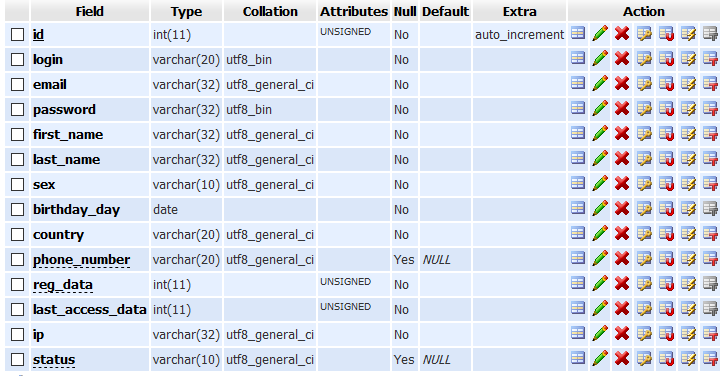
\includegraphics[scale = 0.9]{img/user_tabel}
		\caption{Datele salvate in baza de date}%
		\label{fig:usertabel}
	\end{center}
\end{figure}

\begin{figure}[!htbp]
	\begin{center}
		\centering
		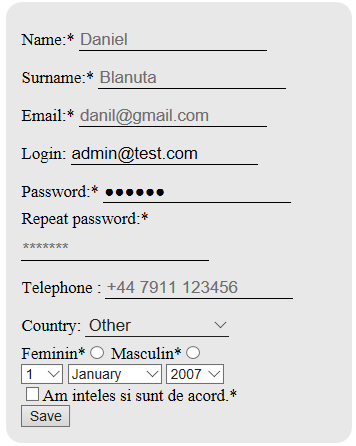
\includegraphics[scale = 0.8]{img/user_form}
		\caption{Forma de inregistrare}%
		\label{fig:add_key_onserver}
	\end{center}
\end{figure}
\begin{figure}[!htbp]
	\begin{center}
		\centering
		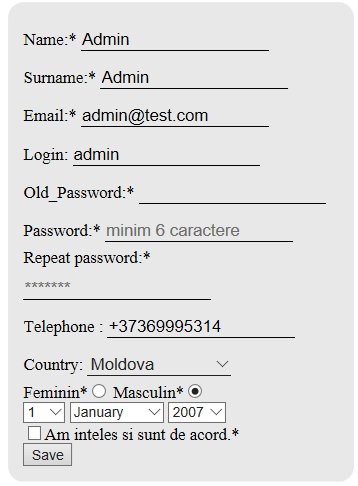
\includegraphics[scale = 0.8]{img/user_data}
		\caption{Forma de corectare a datelor}%
		\label{fig:add_key_onserver}
	\end{center}
\end{figure}

\begin{figure}[!htb]
	\begin{center}
		\centering
		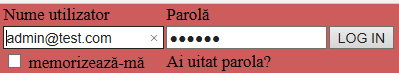
\includegraphics[scale = 0.9]{img/user_login}
		\caption{Forma de logare}%
		\label{fig:git_config}
	\end{center}
\end{figure}

\begin{figure}[htb]
	\begin{center}
		\centering
		
\includegraphics[scale = 0.9]{img/user_panel}
		\caption{User panel}%
		\label{fig:gitinit}
	\end{center}
\end{figure}
\clearpage
